\capitulo{4}{Técnicas y herramientas}
A continuación, a pesar de que se trata de una nueva versión, es decir, modificación y/o mejora de una versión previa, incluiremos todas las técnicas y herramientas utilizadas para el desarrollo de este proyecto.
\section{Android}
Android es un sistema operativo basado en Linux, un núcleo de sistema operativo libre, multiplataforma y gratuito.
Inicialmente Android se creó para teléfono móviles. Actualmente lo podemos encontrar en múltiples dispositivos móviles como tablets, relojes inteligentes, televisores, automóviles…

La estructura del sistema operativo Android se compone de aplicaciones que se ejecutan en un framework Java de aplicaciones orientadas a objetos sobre el núcleo de las bibliotecas de Java en una máquina virtual Dalvik con compilación en tiempo de ejecución hasta la versión 5.0, luego cambió al entorno Android Runtime (ART).
Las bibliotecas escritas en lenguaje C incluyen un administrador de interfaz gráfica (surface manager), un framework OpenCore, una base de datos relacional SQLite, una Interfaz de programación de API gráfica OpenGL ES 2.0 3D, un motor de renderizado WebKit, un motor gráfico SGL, SSL y una biblioteca estándar de C Bionic. El sistema operativo está compuesto por 12 millones de líneas de código, incluyendo 3 millones de líneas de XML, 2.8 millones de líneas de lenguaje C, 2.1 millones de líneas de Java y 1.75 millones de líneas de C++~\cite{wiki:android}.

\subsection{Características}
Características y especificaciones en la actualidad~\cite{wiki:android}.

\begin{table}[]
\centering
\caption{Características y especificaciones 1}
\label{tab:CaracterísticasAndroid1}
\begin{tabular}{@{}
>{\columncolor[HTML]{FFFFFF}}p {.25\textwidth} p {.75\textwidth}@{}}
\toprule
\textbf{Diseño de dispositivo}   & La plataforma es adaptable a pantallas de mayor resolución, VGA, biblioteca de gráficos 2D, biblioteca de gráficos 3D basada en las especificaciones de la OpenGL ES 2.0 y diseño de teléfonos tradicionales.
\\ \midrule
\textbf{Almacenamiento}         & SQLite, una base de datos liviana, que es usada para propósitos de almacenamiento de datos. 
\\ \midrule
\textbf{Conectividad}      & Android soporta las siguientes tecnologías de conectividad: GSM/EDGE, IDEN, CDMA, EV-DO, UMTS, Bluetooth, Wi-Fi, LTE, HSDPA, HSPA+, NFC y WiMAX, GPRS, UMTS y HSDPA+.
 \\ \midrule
\textbf{Mensajería}     & SMS y MMS son formas de mensajería, incluyendo mensajería de texto, además del servicio de Firebase Cloud Messaging (FCM) siendo la nueva versión de Google Cloud Messaging (GCM) bajo la marca Firebase con los nuevos SDK para realizar el desarrollo de mensajería en la nube mucho más sencillo.            
\\ \midrule
\textbf{Navegador web}  & El navegador web incluido en Android está basado en el motor de renderizado de código abierto WebKit, emparejado con el motor JavaScript V8 de Google Chrome. El navegador por defecto de Ice Cream Sandwich obtiene una puntuación de 100/100 en el test Acid3.                                                                                                                                                                        \\ \midrule
\textbf{Soporte de Java}        & Aunque la mayoría de las aplicaciones están escritas en Java, no hay una máquina virtual Java en la plataforma. El bytecode Java no es ejecutado, sino que primero se compila en un ejecutable Dalvik y se ejecuta en la Máquina Virtual Dalvik, Dalvik es una máquina virtual especializada, diseñada específicamente para Android y optimizada para dipositivos móviles que funcionan con batería y que tienen memoria y procesador limitados. A partir de la versión 5.0, se utiliza el Android Runtime (ART). El soporte para J2ME puede ser agregado mediante aplicaciones de terceros como el J2ME MIDP Runner.
\\ \midrule
\textbf{Soporte multimedia} & Android soporta los siguientes formatos multimedia: WebM, H.263, H.264 (en 3GP o MP4), MPEG-4 SP, AMR, AMR-WB (en un contenedor 3GP), AAC, HE-AAC (en contenedores MP4 o 3GP), MP3, MIDI, Ogg Vorbis, WAV, JPEG, PNG, GIF y BMP.                                                                                                                            
\\ \bottomrule
\end{tabular}
\end{table}

\begin{table}[]
\centering
\caption{Características y especificaciones 2}
\label{tab:CaracterísticasAndroid2}
\begin{tabular}{@{}
>{\columncolor[HTML]{FFFFFF}}p {.25\textwidth} p {.75\textwidth}@{}}
\toprule
\textbf{Soporte para streaming}     & Streaming RTP/RTSP (3GPP PSS, ISMA), descarga progresiva de HTML (HTML5 <video> tag). Adobe Flash Streaming (RTMP) es soportado mediante el Adobe Flash Player. Se planea el soporte de Microsoft Smooth Streaming con el port de Silverlight a Android. Adobe Flash HTTP Dynamic Streaming estará disponible mediante una actualización de Adobe Flash Player.
\\ \midrule
\textbf{Soporte para hardware adicional}     & Android soporta cámaras de fotos, de vídeo, pantallas táctiles, GPS, acelerómetros, giroscopios, magnetómetros, sensores de proximidad y de presión, sensores de luz, gamepad, termómetro, aceleración por GPU 2D y 3D.                                                                                                                                                                           
\\ \midrule
\textbf{Entorno de desarrollo}     & Incluye un emulador de dispositivos, herramientas para depuración de memoria y análisis del rendimiento del software. Inicialmente el entorno de desarrollo integrado (IDE) utilizado era Eclipse con el plugin de Herramientas de Desarrollo de Android (ADT). Ahora se considera como entorno oficial Android Studio, descargable desde la página oficial de desarrolladores de Android.
\\ \midrule
\textbf{Google Play}     & Google Play es un catálogo de aplicaciones gratuitas o de pago en el que pueden ser descargadas e instaladas en dispositivos Android sin la necesidad de un PC.
\\ \midrule 
\textbf{Multi-táctil}     & Android tiene soporte nativo para pantallas capacitivas con soporte multitáctil que inicialmente hicieron su aparición en dispositivos como el HTC Hero. La funcionalidad fue originalmente desactivada a nivel de kernel (posiblemente para evitar infringir patentes de otras compañías). Más tarde, Google publicó una actualización para el Nexus One y el Motorola Droid que activa el soporte multitáctil de forma nativa. 
\\ \midrule
\textbf{Bluetooth}     & El soporte para A2DF y AVRCP fue agregado en la versión 1.5;  el envío de archivos (OPP) y la exploración del directorio telefónico fueron agregados en la versión 2.0;  y el marcado por voz junto con el envío de contactos entre teléfonos lo fueron en la versión 2.2.
\\ \midrule
\textbf{Videollamada}     & Android soporta videollamada a través de Hangouts (antiguo Google Talk) desde su versión HoneyComb.
\\ \midrule
\textbf{Multitarea}     & Multitarea real de aplicaciones está disponible, es decir, las aplicaciones que no estén ejecutándose en primer plano reciben ciclos de reloj.
\\ \midrule
\textbf{Características basadas en voz}     & La búsqueda en Google a través de voz está disponible como "Entrada de Búsqueda" desde la versión inicial del sistema.
\\ \bottomrule
\end{tabular}
\end{table}
\subsection{Arquitectura}
\begin{itemize}
	\item\textbf{Aplicaciones}: las aplicaciones base incluyen un cliente de correo electrónico, programa de SMS, calendario, mapas, navegador, contactos y otros. Todas las aplicaciones están escritas en lenguaje de programación Java.
	\item\textbf{Marco de trabajo de aplicaciones}: los desarrolladores tienen acceso completo a los mismas API del entorno de trabajo usados por las aplicaciones base. La arquitectura está diseñada para simplificar la reutilización de componentes; cualquier aplicación puede publicar sus capacidades y cualquier otra aplicación puede luego hacer uso de esas capacidades (sujeto a reglas de seguridad del framework). Este mismo mecanismo permite que los componentes sean reemplazados por el usuario.
	\item\textbf{Bibliotecas}: Android incluye un conjunto de bibliotecas de C/C++ usadas por varios componentes del sistema. Estas características se exponen a los desarrolladores a través del marco de trabajo de aplicaciones de Android. Algunas son: System C library (implementación biblioteca C estándar), bibliotecas de medios, bibliotecas de gráficos, 3D y SQLite, entre otras.
	\item\textbf{Runtime de Android}: Android incluye un set de bibliotecas base que proporcionan la mayor parte de las funciones disponibles en las bibliotecas base del lenguaje Java. Cada aplicación Android corre su propio proceso, con su propia instancia de la máquina virtual Dalvik. Dalvik ha sido escrito de forma que un dispositivo puede correr múltiples máquinas virtuales de forma eficiente. Dalvik ejecutaba hasta la versión 5.0 archivos en el formato de ejecutable Dalvik (.dex), el cual está optimizado para memoria mínima. La Máquina Virtual está basada en registros y corre clases compiladas por el compilador de Java que han sido transformadas al formato.dex por la herramienta incluida dx. Desde la versión 5.0 utiliza el ART, que compila totalmente al momento de instalación de la aplicación.
	\item\textbf{Núcleo Linux}: Android depende de Linux para los servicios base del sistema como seguridad, gestión de memoria, gestión de procesos, pila de red y modelo de controladores. El núcleo también actúa como una capa de abstracción entre el hardware y el resto de la pila de software~\cite{wiki:android}.
\end{itemize}

\begin{figure}
\centering
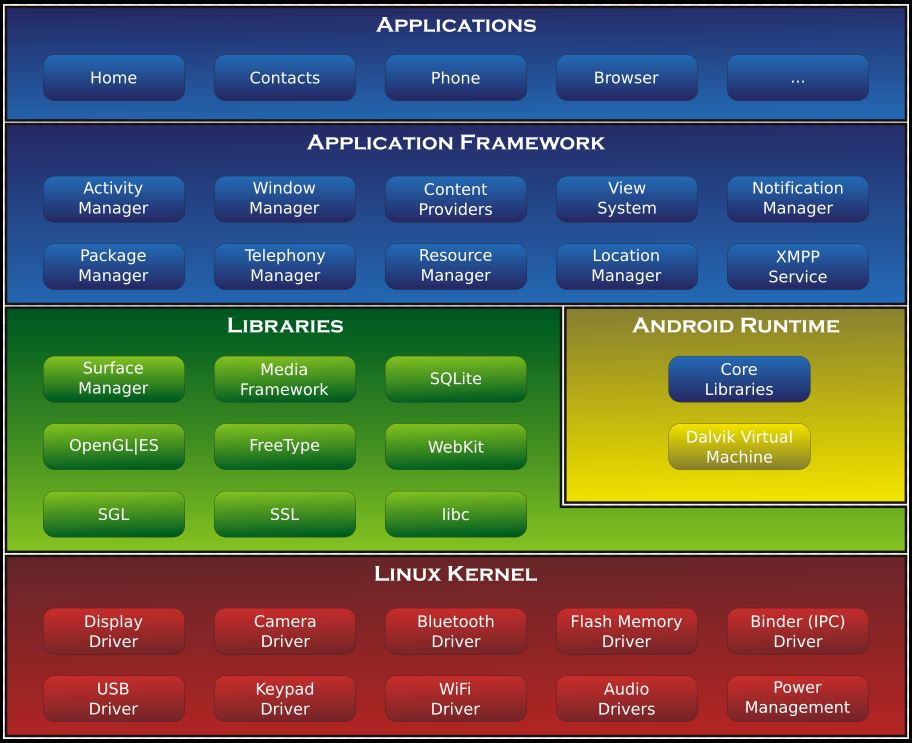
\includegraphics[width=0.95\textwidth]{AndroidSystemArchitecture}
\caption{Arquitectura del sistema Android}
\label{fig:AndroidSystemArchitecture}
\end{figure}

\subsection{Versiones}
Las versiones de Android reciben, en inglés, el nombre de diferentes postres o dulces. En cada versión el postre o dulce elegido empieza por una letra distinta, conforme a un orden alfabético~\cite{wiki:android}:
\begin{table}[]
	\centering
	\caption{Versiones de Android}
	\label{tabla:versionesAndroid}
	\rowcolors {2}{gray!35}{}
	\begin{tabular}{l l l l}
	\toprule
	Letra     & Nombre 		& Versión             & Traducción.\\ 	\midrule    \\ 	
	A         & Apple Pie   & 1.0           	  & Tarta de Manzana.\\ 
	B         & Banana Bread   & 1.1           	  & Pan de plátano.\\ 
	C         & Cupcake   	& 1.0           	  & Cupcake.\\ 
	D         & Donut   	& 1.6           	  & Rosquilla, dónut o Dona.\\ 
	E         & Éclair		& 2.0/2.1             & Pepito o relámpago.\\ 
	F         & Froyo		& 2.0           	  & Yogur helado.\\ 
	G         & Gingerbread & 2.3           	  & Pan de jengibre.\\ 
	H         & Honeycomb   & 3.0/3.1/3.2     	  & Panal.\\ 
	I         & Ice Cream Sandwich    & 4.0       & Sándwich de helado.\\ 
	J         & Jelly Bean    & 4.1/4.2/4.3       & Gominola o pastilla de goma.\\
	K         & KitKat    	& 4.4           	  & KitKat.\\ 
	L         & Lollipop    & 5.0/5.1             & Paleta o Piruleta.\\ 
	M         & Marshmallow & 6.0/6.0.1           & Malvavisco o Bombón o nube.\\ 
	N         & Nougat    	& 7.0/7.1/7.1.1/7.1.2 & Turrón.\\ 
	O         & Oreo    	& 8.0/8.1             & Oreo.\\ 
	P         & P		    & 9.0           	  &  
\\ \bottomrule
\end{tabular}
\end{table}
\newpage
\section{Android Studio}
Android Studio es el entorno de desarrollo integrado oficial para la plataforma Android. Fue anunciado el 16 de mayo de 2013 en la conferencia Google I/O, y reemplazó a Eclipsecomo el IDE oficial para el desarrollo de aplicaciones para Android. La primera versión estable fue publicada en diciembre de 2014.
Está basado en el software IntelliJ IDEA de JetBrains y ha sido publicado de forma gratuita a través de la Licencia Apache 2.0. Está disponible para las plataformas Microsoft Windows, macOS y GNU/Linux. Ha sido diseñado específicamente para el desarrollo de Android.
\subsection{Características}
Las siguientes características se proporcionan en la versión estable actual~\cite{wiki:androidStudio}:
\begin{itemize}
	\item Integración de ProGuard y funciones de firma de aplicaciones.
	\item Renderizado en tiempo real.
	\item Consola de desarrollador: consejos de optimización, ayuda para la traducción, estadísticas de uso.
	\item Soporte para construcción basada en \textbf{Gradle}.
	\item \textbf{Refactorización} específica de Android y arreglos rápidos.
	\item Un editor de diseño enriquecido que permite a los usuarios arrastrar y soltar componentes de la interfaz de usuario.
	\item Herramientas \textbf{Lint} para detectar problemas de rendimiento, usabilidad, compatibilidad de versiones y otros problemas.
	\item Plantillas para crear diseños comunes de Android y otros componentes.
	\item Soporte para programar aplicaciones para \textbf{Android Wear}.
	\item Soporte integrado para Google Cloud Platform, que permite la integración con Google Cloud Messaging y App Engine.
	\item Un dispositivo virtual de Android que se utiliza para ejecutar y probar aplicaciones.
\end{itemize}
\subsection{Plataformas}
Android Studio está disponible para Windows 2003, Vista, 7, 8, y 10, tanto plataformas de 32 como de 64 bits, GNU/Linux, Linux con GNOME o KDE y 2 GB de memoria RAM mínimo y macOS, desde 10.8.5 en adelante~\cite{wiki:androidStudio}.
\subsection{Requisitos del sistema}
 Requisitos del sistema para la plataforma utilizada durante el desarrollo del proyecto: \textbf{Versión 3.x}~\cite{wiki:androidStudio}
 \begin{itemize}
 	\item\textbf{OS Version}: Windows 10/8/7 (32- o 64-bit). 
 	\item\textbf{RAM}: 3 GB RAM mínimo, 8 GB RAM recomendado más 1GB adicional para el emulador de Android.
 	\item\textbf{Espacio en disco}: 2 GB de espacio en disco para Android Studio, 4GB recomendados (500MB para la IDE y al menos 1.5 GB para Android SDK, imágenes de sistema de emulador y cachés).
 	\item\textbf{Java version}: Java Development Kit (JDK) 8.
 	\item\textbf{Resolución de pantalla}: 1280x800 mínimo, 1440x900 recomendado.
 \end{itemize}
\section{AVDManager}
\subsection{¿ Qué significa?}
	AVD Manager (Android Virtual Device Manager) es un gestor para los dispositivos virtuales de Android, es decir, los emuladores. 
\subsection{¿ Para qué sirve ?}
Para crear y gestionar los emuladores de Android en los que se probaran las aplicaciones. Estos emuladores pueden ser creados con perfiles predefinidos de dispositivos de fabricantes reales, o con características propias personalizadas por el programador.
\subsection{¿ Cómo se Configura ?}
\begin{itemize}
	\item Tools> AVD Manager.
	\item Clic en el botón ``+ Create Virtual Device''.
	\item Seleccionamos la categoría del dispositivo virtual que queremos crear: \textbf{Phone}.
	\item Seleccionamos un fabricante con las características deseadas.
	\item Clic en el botón ``Next''.
	\item Seleccionamos la versión del sistema operativo que queremos usar. Si no está disponible, se puede descargar cualquier versión haciendo clic en ``Download''.
	\item Clic en el botón ``Next''.
	\item Verificamos la configuración del emulador que se va a crear. Se puede editar la configuración recomendada haciendo clic en el botón ``Show Advanced Settings''.
	\item Clic en el botón ``Finish''.
\end{itemize}
\subsection{¿ Cómo se utiliza ?}
Para poder ejecutar nuestra aplicación en un emulador, desde la ventana AVD Manager seleccionamos un emulador (previamente creado) y en la pestaña \textbf{Actions} hacemos clic en el botón ``Play''.

\section{SDK}
El SDK (Software Development Kit) de Android, incluye un conjunto de herramientas de desarrollo. Comprende un depurador de código, biblioteca, un simulador de teléfono basado en QEMU, documentación, ejemplos de código y tutoriales. Las plataformas de desarrollo soportadas incluyen GNU/Linux, Mac OS X 10.5.8 o posterior, y Windows XP o posterior. La plataforma integral de desarrollo (IDE, Integrated Development Environment) soportada oficialmente es Android Studio junto con el complemento ADT ( Android Development Tools plugin). Además, los programadores pueden usar un editor de texto para escribir ficheros Java y XML y utilizar comandos en un terminal (se necesitan los paquetes JDK, Java Development Kit y Apache Ant) para crear y depurar aplicaciones, así como controlar dispositivos Android que estén conectados ( es decir, reiniciarlos, instalar aplicaciones en remoto, etc.). 
Las Actualizaciones del SDK están coordinadas con el desarrollo general de Android. El SDK soporta también versiones antiguas de Android, por si los programadores necesitan instalar aplicaciones en dispositivos ya obsoletos o más antiguos. Las herramientas de desarrollo son componentes descargables, de modo que una vez instalada la última versión, pueden instalarse versiones anteriores y hacer pruebas de compatibilidad~\cite{wiki:androidsdk}. 

\section{SQLite}
\subsection{¿ Qué es SQLite ?}
SQLite es una base de datos de código abierto que está integrada en Android. SQLite admite estándar características de bases de datos relacionales como sintaxis SQL, transacciones y declaraciones preparadas. Además, requiere solo poca memoria en tiempo de ejecución (aproximadamente 250 KByte). SQLite admite los tipos de datos TEXT (similar a String en Java), INTEGER (similar a long en Java) y REAL (similar al doble en Java). Todos los demás tipos deben convertirse en uno de estos campos antes guardándolos en la base de datos. SQLite en sí no valida si los tipos escritos en las columnas son en realidad del tipo definido, p. puedes escribir un entero en una columna de cadena y viceversa. Se puede encontrar más información sobre SQLite en el sitio web de SQLite: http://www.sqlite.org~\cite{vogel2010android}.
\subsection{SQLite en Android}
SQLite está disponible en todos los dispositivos Android. El uso de una base de datos SQLite en Android no requiere ninguna configuración o administración de base de datos.
Solo debe definir las instrucciones SQL para crear y actualizar la base de datos. Luego, la plataforma Android administrará automáticamente la base de datos.
El acceso a una base de datos SQLite implica el acceso al sistema de archivos. Esto puede ser lento. Por lo tanto, se recomienda realizar operaciones de base de datos de forma asincrónica, por ejemplo, dentro de la clase AsyncTask. Si su aplicación crea una base de datos, esta base de datos se guarda de manera predeterminada en el directorio ``DATA\/data\/ APP\/NAME\/databases\/FILENAME''. Las partes del directorio anterior se construyen en base a las siguientes reglas. \textbf{DATA} es el camino que el método Environment.getDataDirectory() devuelve.\textbf{APP\_NAME} es el nombre de tu aplicación.\textbf{FILENAME} es el nombre que especificas en tu código de aplicación para la base de datos.

\section{DB Browser for SQLite}
En este proyecto, DB Browser for SQLite se ha utilizado básicamente para comprobar que los datos creados o registrados en nuestra base da datos (desde nuestra aplicación) son correctos.
\subsection{¿ Qué es ?}
DB Browser for SQLite es una herramienta de alta calidad, visual y de código abierto para crear, diseñar y editar archivos de bases de datos compatibles con SQLite. Es para usuarios y desarrolladores que desean crear bases de datos, buscar y editar datos. Utiliza una interfaz familiar similar a una hoja de cálculo, y no necesita aprender comandos SQL complicados. Los controles y asistentes están disponibles para que los usuarios~\cite{sqlitebrowser}:
\begin{itemize}
	\item Crear y compactar archivos de base de datos.
	\item Crear, definir, modificar y eliminar tablas.
	\item Crear, definir y eliminar índices.
	\item Examinar, editar, agregar y eliminar registros.
	\item Registros de búsqueda.
	\item Importar y exportar registros como texto.
	\item Importar y exportar tablas de / a archivos CSV.
	\item Importar y exportar bases de datos desde / a archivos de volcado de SQL.
	\item Emita consultas SQL e inspeccione los resultados.
	\item Examine un registro de todos los comandos SQL emitidos por la aplicación.

\end{itemize}
\subsection{¿ Qué no es?}
Este programa no es un shell visual para la herramienta de línea de comandos sqlite. No requiere familiaridad con los comandos SQL. Es una herramienta para ser utilizada tanto por los desarrolladores como por los usuarios finales, y debe ser tan simple de usar como sea posible para alcanzar sus objetivos~\cite{sqlitebrowser}.
\section{Java}
Java es un lenguaje de programación de propósito general, concurrente, orientado a objetos, que fue diseñado específicamente para tener tan pocas dependencias de implementación como fuera posible. Su intención es permitir que los desarrolladores de aplicaciones escriban el programa una vez y lo ejecuten en cualquier dispositivo (conocido en inglés como WORA, o "write once, run anywhere"), lo que quiere decir que el código que es ejecutado en una plataforma no tiene que ser recompilado para correr en otra. Java es, a partir de 2012, uno de los lenguajes de programación más populares en uso, particularmente para aplicaciones de cliente-servidor de web, con unos diez millones de usuarios reportados~\cite{wiki:java}. 
Webs de la herramienta:
\begin{itemize}
	\item https://www.oracle.com/java/index.html
	\item https://www.java.com/es/download/
\end{itemize}
\section{JUnit}

JUnit es un conjunto de bibliotecas creadas por Erich Gamma y Kent Beck que son utilizadas en programación para hacer pruebas unitarias de aplicaciones Java.
JUnit es un conjunto de clases (framework) que permite realizar la ejecución de clases Java de manera controlada, para poder evaluar si el funcionamiento de cada uno de los métodos de la clase se comporta como se espera. Es decir, en función de algún valor de entrada se evalúa el valor de retorno esperado; si la clase cumple con la especificación, entonces JUnit devolverá que el método de la clase pasó exitosamente la prueba; en caso de que el valor esperado sea diferente al que regresó el método durante la ejecución, JUnit devolverá un fallo en el método correspondiente.
JUnit es también un medio de controlar las pruebas de regresión, necesarias cuando una parte del código ha sido modificado y se desea ver que el nuevo código cumple con los requerimientos anteriores y que no se ha alterado su funcionalidad después de la nueva modificación~\cite{wiki:junit}.
\subsection{JUnit en Android Studio}
Desde la versión 1.1 de Android Studio existe, lo que han llamado desde google, soporte para test unitarios. Esto quiere decir que podemos ejecutar test unitarios sin necesidad de desplegar en un dispositivo o emulador, se van a ejecutar en la máquina virtual de java. 

Estos test untarios se conocen también como test locales o test de jvm (java virtual machine). 


\section{Espresso}
Espresso es un framework de testing open source lanzado por Google el cual provee una API que permite crear pruebas de interfaz de usuario (de ahora en adelante UI por sus siglas en inglés) para simular interacciones de usuarios en una aplicación Android (en la versión 2.2 en adelante). Es una buena práctica simular los diferentes escenarios en los que el usuario puede interacturar con una aplicación para evitar que este se encuentre con resultados inesperados o bien tenga una mala experiencia al momento de su uso. Es por esta razón que es recomendable la creación de un entorno de pruebas vinculadas a la UI con el fin de asegurarnos que la aplicación está funcionando correctamente.
Su principal ventaja es que nos permite la sincronización automática de las acciones de las pruebas con la interfaz de usuario de nuestra aplicación. Además, permite la ejecución de pruebas en máquinas x86 en un ambiente multihilo, solucionando problemas de concurrencia asociados al testing de UI.
Espresso permite realizar pruebas tanto en dispositivos físicos como virtuales (emuladores)~\cite{wiki:espresso}.

\section{Git}
Git es un software de control de versiones diseñado por Linus Torvalds, pensando en la eficiencia y la confiabilidad del mantenimiento de versiones de aplicaciones cuando éstas tienen un gran número de archivos de código fuente. Su propósito es llevar registro de los cambios en archivos de computadora y coordinar el trabajo que varias personas realizan sobre archivos compartidos.
Al principio, Git se pensó como un motor de bajo nivel sobre el cual otros pudieran escribir la interfaz de usuario o front end como Cogito o StGIT.  Sin embargo, Git se ha convertido desde entonces en un sistema de control de versiones con funcionalidad plena.  Hay algunos proyectos de mucha relevancia que ya usan Git, en particular, el grupo de programación del núcleo Linux.
El mantenimiento del software Git está actualmente (2009) supervisado por Junio Hamano, quien recibe contribuciones al código de alrededor de 280 programadores. En cuanto a derechos de autor Git es un software libre distribuible bajo los términos de la versión 2 de la Licencia Pública General de GNU~\cite{wiki:git}.
\subsection{Características}
El diseño de Git mantiene una enorme cantidad de código distribuida y gestionada por mucha gente, que incide en numerosos detalles de rendimiento, y de la necesidad de rapidez en una primera implementación.
Entre las características más relevantes se encuentran:
\begin{itemize}
	\item Fuerte apoyo al desarrollo no lineal, por ende, rapidez en la gestión de ramas y mezclado de diferentes versiones. Git incluye herramientas específicas para navegar y visualizar un historial de desarrollo no lineal. Una presunción fundamental en Git es que un cambio será fusionado mucho más frecuentemente de lo que se escribe originalmente, conforme se pasa entre varios programadores que lo revisan.
	\item Gestión distribuida. Al igual que Darcs, BitKeeper, Mercurial, SVK, Bazaar y Monotone, Git le da a cada programador una copia local del historial del desarrollo entero, y los cambios se propagan entre los repositorios locales. Los cambios se importan como ramas adicionales y pueden ser fusionados en la misma manera que se hace con la rama local.
	\item Los almacenes de información pueden publicarse por HTTP, FTP, rsync o mediante un protocolo nativo, ya sea a través de una conexión TCP/IP simple o a través de cifrado SSH. Git también puede emular servidores CVS, lo que habilita el uso de clientes CVS pre-existentes y módulos IDE para CVS pre-existentes en el acceso de repositorios Git.
	\item Los repositorios Subversion y svk se pueden usar directamente con git-svn.
	\item Gestión eficiente de proyectos grandes, dada la rapidez de gestión de diferencias entre archivos, entre otras mejoras de optimización de velocidad de ejecución.
	\item Todas las versiones previas a un cambio determinado implican la notificación de un cambio posterior en cualquiera de ellas a ese cambio (denominado autenticación criptográfica de historial). Esto existía en Monotone.
	\item Resulta algo más caro trabajar con ficheros concretos frente a proyectos, eso diferencia el trabajo frente a CVS, que trabaja con base en cambios de fichero, pero mejora el trabajo con afectaciones de código que concurren en operaciones similares en varios archivos.
	\item Los renombrados se trabajan basándose en similitudes entre ficheros, aparte de nombres de ficheros, pero no se hacen marcas explícitas de cambios de nombre con base en supuestos nombres únicos de nodos de sistema de ficheros, lo que evita posibles, y posiblemente desastrosas, coincidencias de ficheros diferentes en un único nombre.
	\item Realmacenamiento periódico en paquetes (ficheros). Esto es relativamente eficiente para escritura de cambios y relativamente ineficiente para lectura si el reempaquetado (con base en diferencias) no ocurre cada cierto tiempo.	
\end{itemize}
\section{GitHub-Desktop}
GitHub es una plataforma de alojamiento de código para control de versiones y colaboración. En otras palabras, GitHub es un alojamiento de repositorios Git que nos permite trabajar en proyectos desde cualquier lugar~\cite{gitHub}.

GitHub Desktop es una aplicación de escritorio de GitHub que nos permite empezar a utilizar un control de versiones sin problemas. GitHub Desktop es una interfaz gráfica de usuario diseñada para facilitar el uso de Git, es decir, permite al usuario interactuar con el programa a través de un dispositivo visual que reemplaza la línea de comandos.

\section{Latext}
Latext es un sistema de composición de textos, orientado a la creación de documentos escritos que presenten una alta calidad tipográfica. Por sus características y posibilidades, es usado de forma especialmente intensa en la generación de artículos y libros científicos que incluyen, entre otros elementos, expresiones matemáticas.
LaTeX está formado por un gran conjunto de macros de TeX, escrito por Leslie Lamport en 1984, con la intención de facilitar el uso del lenguaje de composición tipográfica, TEX, creado por Donald Knuth. Es muy utilizado para la composición de artículos académicos, tesis y libros técnicos, dado que la calidad tipográfica de los documentos realizados en LaTeX, se la considera adecuada a las necesidades de una editorial científica de primera línea, muchas de las cuales ya lo emplean.
LaTeX es software libre bajo licencia LPPL~\cite{wiki:latex}.

\section{Texmaker}
Texmaker es un editor gratuito distribuido bajo la licencia GPL para escribir documentos de texto, multiplataforma, que integra muchas herramientas necesarias para desarrollar documentos con LaTeX, en una sola aplicación. Texmaker incluye soporte Unicode, corrección ortográfica, auto-completado, plegado de código y un visor incorporado en pdf con soporte de synctex y el modo de visualización continua.
Para que Texmaker pueda funcionar es necesario haber instalado TeX previamente~\cite{wiki:texmaker}.

\section{Photoshop CC 2017}
Adobe Photoshop es un editor de gráficos rasterizados desarrollado por Adobe Systems Incorporated. Usado principalmente para el retoque de fotografías y gráficos, su nombre en español significa literalmente``taller de fotos''. Es líder mundial del mercado de las aplicaciones de edición de imágenes y domina este sector de tal manera que su nombre es ampliamente empleado como sinónimo para la edición de imágenes en general~\cite{wiki:adobephotoshop}. 
En el desarrollo de este proyecto, se ha utilizado Adobe Photoshop CC 2017 únicamente para la creación y edición del icono de la app.
